\documentclass[11pt,a4paper]{ltxdoc}
\usepackage[margin=2cm]{geometry}

\usepackage[libertine]{newtxmath}
\usepackage[oldstyle]{libertine}
\usepackage{fontspec}
\setmonofont[Scale=0.82]{MesloLGS-Regular.ttf}[
  BoldFont=MesloLGS-Bold.ttf,
  ItalicFont=MesloLGS-Italic.ttf,
  BoldItalicFont=MesloLGS-BoldItalic.ttf
]

\usepackage[colorlinks]{hyperref}

\usepackage[svgnames,table,hyperref]{xcolor}
\usepackage{minted}
\usepackage[all]{tcolorbox}
\tcbset{
  listing engine=minted,
  skin=enhanced,
  before doc body={\setlength\parskip{1ex}\normalsize},
  docexample/.style=
    {colframe=ExampleFrame,colback=ExampleBack,before skip=\medskipamount,
    sharp corners,enhanced,boxrule=0pt,overlay={
    \draw[ExampleFrame] (frame.north west) rectangle (frame.south east);}},%after skip=\medskipamount
  doc head={colback=yellow!10!white,interior style=fill},
  doc head key={colback=magenta!5!white,interior style=fill},
  doc head path={colback=blue!50!gray!7!white,interior style=fill},
  color key=DarkViolet,
  color value=Teal,
  color color=Teal,
  color counter=Orange!85!black,
  color length=Orange!85!black
}

\usepackage{tikzmusic}
\usepackage{pgfplots}
\pgfplotsset{compat=1.16}

\usepackage{fancyvrb}
\DefineShortVerb{\|}

\setlength\parindent{0pt}

\newcommand\pkg[1]{{\sffamily #1}}
\newcommand\tmname{\pkg{tikzmusic}}
\newcommand\tikzname{Ti\emph{k}Z}

\newtcolorbox{caution}{
  enhanced,
  before skip=2mm,after skip=3mm,
  boxrule=0pt,frame hidden,left=6mm,right=1mm,top=1mm,bottom=1mm,
  colback=yellow!10,colframe=yellow,sharp corners,
  underlay={
    \path[fill=yellow,draw=none] 
      (interior.south west) rectangle node {\Huge\bfseries !} ([xshift=5mm]interior.north west);
  },
  overlay={
    \draw[yellow] (frame.north west) rectangle (frame.south east);
  }
}

\makeindex

\title{The \tmname\ package}
\author{Vũ Văn Dũng}
\date{Last compiled: \today}
\begin{document}
\maketitle
\begin{abstract}
  This package will help you make music scores inside a \LaTeX\ document. All 
  drawings will be done by the amazing \tikzname\ package.
\end{abstract}
\begin{caution}
  This package is still very experimental, uncompleted and lack of many important 
  features. Its syntax can change at any time. Only use it if you have good 
  reasons.
\end{caution}
\tableofcontents
\setlength\parskip{1ex}
\section{Initialization}\label{sec:init}
\subsection{Loading the package}\label{sec:init:load}
This package currently only supports \LaTeX.

There are no options. Hence, to load the package, you just need to 
include the following line
\begin{dispListing}
\usepackage{tikzmusic}
\end{dispListing}
inside your document preamble.

This package will automatically load the the packages \pkg{xparse}, \pkg{etoolbox}, 
\pkg{xstring} and \tikzname, as well as \tikzname\ standard libraries |calc|, 
|intersection|, |decorations.pathreplacing|. The \tikzname\ library |calligraphy| 
is also loaded. You don't need to load these packages and libraries again in your 
document.
\subsection{Environments for music lines}\label{sec:init:drawing-environment}
Each score line will be drawn separately. Depending on the number of staves you 
want in each line, you have two options:

\begin{docEnvironment}[doclang/environment content=music line]{tmsinglestaff}{}
  If you have only one staff per line, you should use this environment. 
  Every drawing in \tmname\ should be done in this environment.
\end{docEnvironment}
\begin{docEnvironment}[doclang/environment content=music line]{tmmultiplestaves}{\oarg{offset}}
  In case you have more than two staves per line (e.g. when you are writing a 
  piano piece), you should use this environment to contain each of your lines. 
  The staves will not start from the left margin of the paper, but leave a 
  horizontal space of \meta{offset} for the braces and brackets. \meta{offset} 
  is $2$cm by default.
\end{docEnvironment}
\subsection{Creating a staff}\label{sec:init:staff-creation}
A staff can be created using one of the following environments:
\begin{docEnvironment}[doclang/environment content=drawing commands]{tmstaff}{\marg{clef name}\oarg{staff name}}
  Create a staff, with the starting clef is \meta{clef name}.

  \meta{clef name} can have three values: |g|, |f| and |c|, which stands for 
  the treble (G) clef, the bass (F) clef and the alto (C) clef, respectively.

  \meta{staff name} will be used to make cross-staff barlines or braces, so 
  even though you can left it empty, you really shouldn't do so.

  The starting point of the staff (as demonstrated below) is named as coordinate 
  |(|\meta{staff name}|-start)|, which you can use later with 
  |remember picture,overlay| \tikzname\ pictures.
\end{docEnvironment}
\begin{dispExample}
\begin{tmsinglestaff}%
  \begin{tmstaff}{g}[my-staff]
  \end{tmstaff}%
  \tikz[remember picture,overlay] \fill[red] (my-staff-start) circle (1.5pt);%
\end{tmsinglestaff}
\end{dispExample}
\begin{docEnvironment}[doclang/environment content=drawing commands]{tmstaff*}{\oarg{staff name}}
  Work like \refEnv*{tmstaff}, but no clefs will be drawn.
\end{docEnvironment}
Essentially, \refEnv*{tmstaff} and \refEnv*{tmstaff*} are extensions of the 
|tikzpicture| environment. 

\section{Multiple-staff operations}\label{sec:multistaff}
Because the following commands are multiple-staff commands, they should be 
used outside \refEnv*{tmstaff} and \refEnv*{tmstaff*} (\emph{except} 
\refCom*{tmbarlineinline}, \refCom*{tmdoublebarlineinline}, \dots).
\subsection{Ensembling staves}\label{sec:multistaff:ensemble-staves}
Braces that groups some staves inside a \refEnv*{tmmultiplestaves} can be drawn 
using the following command:
\begin{docCommand}{tmbrace}{\marg{uppermost staff name}\marg{lowermost staff name}\marg{middle text}}
  Draw a brace spanning from \meta{uppermost staff name} to \meta{lowermost staff name}. 
  \meta{middle text} is displayed at the middle of the brace. If you don't want 
  any text to be displayed, you can leave this option empty.
\end{docCommand}
\begin{dispExample}
\begin{tmmultiplestaves}%
  \begin{tmstaff}{g}[piano-1]
  \end{tmstaff}%
  \begin{tmstaff}{f}[piano-2]
  \end{tmstaff}%
  \tmbrace{piano-1}{piano-2}{Piano}%
\end{tmmultiplestaves}
\end{dispExample}

Similarly, brackets can also be drawn:

\begin{docCommand}{tmbracket}{\marg{uppermost staff name}\marg{lowermost staff name}}
  Draw a bracket spanning from \meta{uppermost staff name} to \meta{lowermost staff name}. 
  Unlike \refCom*{tmbrace}, no text will be displayed.
\end{docCommand}
\begin{dispExample}
\begin{tmmultiplestaves}%
  \begin{tmstaff}{g}[Violin]
  \end{tmstaff}%
  \begin{tmstaff}{c}[Viola]
  \end{tmstaff}%
  \begin{tmstaff}{f}[Violoncello]
  \end{tmstaff}%
  \foreach \i in {Violin,Viola,Violoncello}%
    {\tikz[remember picture,overlay] \path (\i-start) node[left=2mm] {\i};}%
  \tmbracket{Violin}{Violoncello}%
\end{tmmultiplestaves}
\end{dispExample}
\subsection{Barlines}\label{sec:multistaff:barlines}
The \tmname\ package supports many different types of barlines. 

\subsubsection{Normal barlines}\label{sec:multistaff:barlines:normal}
\begin{docCommand}{tmbarline}{\marg{x-pos}\marg{staff name}}
  Draw a normal barline on \meta{staff name} at $x$-position \meta{x-pos} in 
  relative to the starting coordinate |(|\meta{staff name}|-start)|.
\end{docCommand}
\begin{dispExample}
\begin{tmmultiplestaves}[0pt]%
  \begin{tmstaff}{g}[staff-1]
  \end{tmstaff}%
  \begin{tmstaff}{f}[staff-2]
  \end{tmstaff}%
  \tmbarline{5}{staff-1}%
  \tmbarline{5}{staff-2}%
\end{tmmultiplestaves}
\end{dispExample}
\begin{docCommand}{tmbarline*}{\marg{x-pos}\marg{uppermost staff name}\marg{lowermost staff name}}
  Draw a normal barline spanning from \meta{uppermost staff name} to 
  \meta{lowermost staff name}, at $x$-position \meta{x-pos} in relative to 
  the starting coordinate |(|\meta{staff name}|-start)| of either staff.
\end{docCommand}
\begin{dispExample}
\begin{tmmultiplestaves}[0pt]%
  \begin{tmstaff}{g}[staff-1]
  \end{tmstaff}%
  \begin{tmstaff}{c}[staff-2]
  \end{tmstaff}%
  \begin{tmstaff}{f}[staff-3]
  \end{tmstaff}%
  \tmbarline*{5}{staff-1}{staff-3}%
\end{tmmultiplestaves}
\end{dispExample}

A special case of \refCom*{tmbarline*} is implemented in the following command:
\begin{docCommand}{tmbarlineendline}{\marg{uppermost staff name}\marg{lowermost staff name}}
  Draw a normal barline spanning from \meta{uppermost staff name} to 
  \meta{lowermost staff name} at the end of the line.
\end{docCommand}
\begin{dispExample}
\begin{tmmultiplestaves}[0pt]%
  \begin{tmstaff}{g}[staff-1]
  \end{tmstaff}%
  \begin{tmstaff}{c}[staff-2]
  \end{tmstaff}%
  \begin{tmstaff}{f}[staff-3]
  \end{tmstaff}%
  \tmbarline*{0}{staff-1}{staff-3}%
  \tmbarlineendline{staff-1}{staff-3}%
\end{tmmultiplestaves}
\end{dispExample}

If you want to draw the barline inside \refEnv*{tmstaff} or \refEnv*{tmstaff*}, 
you can use 
\begin{docCommand}{tmbarlineinline}{\marg{list of x-pos}}
  Draw a normal barline at each $x$-position specified in \marg{list of x-pos}.
\end{docCommand}
\begin{dispExample}
\begin{tmsinglestaff}%
  \begin{tmstaff}{g}[]
    \tmbarlineinline{3,5,8,9}
  \end{tmstaff}%
\end{tmsinglestaff}
\end{dispExample}
\subsubsection{Double barlines}\label{sec:multistaff:barlines:double}
Like when drawing normal barlines as described in Section 
\ref{sec:multistaff:barlines:normal} on page \pageref{sec:multistaff:barlines:normal}, 
we also have four commands for double barlines.

\begin{docCommand}{tmdoublebarline}{\marg{x-pos}\marg{staff name}}
  Draw a double barline on \meta{staff name} at $x$-position \meta{x-pos} in 
  relative to the starting coordinate |(|\meta{staff name}|-start)|.
\end{docCommand}
\begin{docCommand}{tmdoublebarline*}{\marg{x-pos}\marg{uppermost staff name}\marg{lowermost staff name}}
  Draw a double barline spanning from \meta{uppermost staff name} to 
  \meta{lowermost staff name}, at $x$-position \meta{x-pos} in relative to 
  the starting coordinate |(|\meta{staff name}|-start)| of either staff.
\end{docCommand}
\begin{docCommand}{tmdoublebarlineendline}{\marg{uppermost staff name}\marg{lowermost staff name}}
  Draw a double barline spanning from \meta{uppermost staff name} to 
  \meta{lowermost staff name} at the end of the line.
\end{docCommand}
\begin{docCommand}{tmdoublebarlineinline}{\marg{list of x-pos}}
  Draw a double barline at each $x$-position specified in \marg{list of x-pos}.
\end{docCommand}
Example use of all four commands described in this section:
\begin{dispExample}
\begin{tmmultiplestaves}[0pt]%
  \begin{tmstaff}{g}[staff-1]
  \end{tmstaff}%
  \begin{tmstaff}{c}[staff-2]
  \end{tmstaff}%
  \begin{tmstaff}{f}[staff-3]
    \tmdoublebarlineinline{8,9,10}
  \end{tmstaff}%
  \tmbarline*{0}{staff-1}{staff-3}%
  \tmdoublebarline*{4}{staff-1}{staff-3}%
  \tmdoublebarline{7}{staff-1}%
  \tmdoublebarlineendline{staff-1}{staff-3}%
\end{tmmultiplestaves}
\end{dispExample}


\subsubsection{Dotted barlines}\label{sec:multistaff:barlines:dotted}
Now you can see the patterns :).

\begin{docCommand}{tmdottedbarline}{\marg{x-pos}\marg{staff name}}
  Draw a dotted barline on \meta{staff name} at $x$-position \meta{x-pos} in 
  relative to the starting coordinate |(|\meta{staff name}|-start)|.
\end{docCommand}
\begin{docCommand}{tmdottedbarline*}{\marg{x-pos}\marg{uppermost staff name}\marg{lowermost staff name}}
  Draw a dotted barline spanning from \meta{uppermost staff name} to 
  \meta{lowermost staff name}, at $x$-position \meta{x-pos} in relative to 
  the starting coordinate |(|\meta{staff name}|-start)| of either staff.
\end{docCommand}
\begin{docCommand}{tmdottedbarlineendline}{\marg{uppermost staff name}\marg{lowermost staff name}}
  Draw a dotted barline spanning from \meta{uppermost staff name} to 
  \meta{lowermost staff name} at the end of the line.
\end{docCommand}
\begin{docCommand}{tmdottedbarlineinline}{\marg{list of x-pos}}
  Draw a double barline at each $x$-position specified in \marg{list of x-pos}.
\end{docCommand}
The commands in use:
\begin{dispExample}
\begin{tmmultiplestaves}[0pt]%
  \begin{tmstaff}{g}[staff-1]
  \end{tmstaff}%
  \begin{tmstaff}{c}[staff-2]
  \end{tmstaff}%
  \begin{tmstaff}{f}[staff-3]
    \tmdottedbarlineinline{8,9,10}
  \end{tmstaff}%
  \tmbarline*{0}{staff-1}{staff-3}%
  \tmdottedbarline*{4}{staff-1}{staff-3}%
  \tmdottedbarline{7}{staff-1}%
  \tmdottedbarlineendline{staff-1}{staff-3}%
\end{tmmultiplestaves}
\end{dispExample}

\subsubsection{Final barlines}\label{sec:multistaff:barlines:final}
\begin{docCommand}{tmfinalbarline}{\marg{x-pos}\marg{staff name}}
  Draw a final barline on \meta{staff name} at $x$-position \meta{x-pos} in 
  relative to the starting coordinate |(|\meta{staff name}|-start)|.
\end{docCommand}
\begin{docCommand}{tmfinalbarline*}{\marg{x-pos}\marg{uppermost staff name}\marg{lowermost staff name}}
  Draw a final barline spanning from \meta{uppermost staff name} to 
  \meta{lowermost staff name}, at $x$-position \meta{x-pos} in relative to 
  the starting coordinate |(|\meta{staff name}|-start)| of either staff.
\end{docCommand}
\begin{docCommand}{tmfinalbarlineendline}{\marg{uppermost staff name}\marg{lowermost staff name}}
  Draw a final barline spanning from \meta{uppermost staff name} to 
  \meta{lowermost staff name} at the end of the line.
\end{docCommand}
\begin{docCommand}{tmfinalbarlineinline}{\marg{list of x-pos}}
  Draw a final barline at each $x$-position specified in \marg{list of x-pos}.
\end{docCommand}
\begin{dispExample}
\begin{tmmultiplestaves}[0pt]%
  \begin{tmstaff}{g}[staff-1]
  \end{tmstaff}%
  \begin{tmstaff}{c}[staff-2]
  \end{tmstaff}%
  \begin{tmstaff}{f}[staff-3]
    \tmfinalbarlineinline{8,9,10}
  \end{tmstaff}%
  \tmbarline*{0}{staff-1}{staff-3}%
  \tmfinalbarline*{4}{staff-1}{staff-3}%
  \tmfinalbarline{7}{staff-1}%
  \tmfinalbarlineendline{staff-1}{staff-3}%
\end{tmmultiplestaves}
\end{dispExample}

\subsubsection{Start repeat barlines}\label{sec:multistaff:barlines:start}
\begin{docCommand}{tmstartrepeatbarline}{\marg{x-pos}\marg{staff name}}
  Draw a start repeat barline on \meta{staff name} at $x$-position \meta{x-pos} in 
  relative to the starting coordinate |(|\meta{staff name}|-start)|.
\end{docCommand}
\begin{docCommand}{tmstartrepeatbarline*}{\marg{x-pos}\marg{uppermost staff name}\marg{lowermost staff name}\marg{list of staff names}}
  Draw a start repeat barline spanning from \meta{uppermost staff name} to 
  \meta{lowermost staff name}, at $x$-position \meta{x-pos} in relative to 
  the starting coordinate |(|\meta{staff name}|-start)| of either staff.

  Because of some internal problems, you need to specify a full list of the names 
  of the staff that the barline spans over in \meta{list of staff names} with 
  a standard comma-separated list.
\end{docCommand}
\begin{docCommand}{tmstartrepeatbarlineinline}{\marg{list of x-pos}}
  Draw a start repeat barline at each $x$-position specified in \marg{list of x-pos}.
\end{docCommand}
\begin{dispExample}
\begin{tmmultiplestaves}[0pt]%
  \begin{tmstaff}{g}[staff-1]
  \end{tmstaff}%
  \begin{tmstaff}{c}[staff-2]
  \end{tmstaff}%
  \begin{tmstaff}{f}[staff-3]
    \tmstartrepeatbarlineinline{8,9,10}
  \end{tmstaff}%
  \tmbarline*{0}{staff-1}{staff-3}%
  \tmstartrepeatbarline*{4}{staff-1}{staff-3}{staff-1,staff-2,staff-3}%
  \tmstartrepeatbarline{7}{staff-1}%
\end{tmmultiplestaves}
\end{dispExample}
\begin{caution}
  Note that there is no \cs{tmstartrepeatbarlineendline}, because I am sure you 
  will never put a start repeat barline to the end of a line.
\end{caution}
\subsubsection{End repeat barlines}\label{sec:multistaff:barlines:end}
\begin{docCommand}{tmendrepeatbarline}{\marg{x-pos}\marg{staff name}}
  Draw an end repeat barline on \meta{staff name} at $x$-position \meta{x-pos} in 
  relative to the starting coordinate |(|\meta{staff name}|-start)|.
\end{docCommand}
\begin{docCommand}{tmendrepeatbarline*}{\marg{x-pos}\marg{uppermost staff name}\marg{lowermost staff name}\marg{list of staff names}}
  Draw an end repeat barline spanning from \meta{uppermost staff name} to 
  \meta{lowermost staff name}, at $x$-position \meta{x-pos} in relative to 
  the starting coordinate |(|\meta{staff name}|-start)| of either staff.

  Similar to \refCom*{tmstartrepeatbarline*}, you also need to specify 
  \meta{list of staff names.}
\end{docCommand}
\begin{docCommand}{tmendrepeatbarlineendline}{\marg{uppermost staff name}\marg{lowermost staff name}\marg{list of staff names}}
  Draw an end repeat barline spanning from \meta{uppermost staff name} to 
  \meta{lowermost staff name} at the end of the line. 
\end{docCommand}
\begin{docCommand}{tmendrepeatbarlineinline}{\marg{list of x-pos}}
  Draw a end repeat barline at each $x$-position specified in \marg{list of x-pos}.
\end{docCommand}
\begin{dispExample}
\begin{tmmultiplestaves}[0pt]%
  \begin{tmstaff}{g}[staff-1]
  \end{tmstaff}%
  \begin{tmstaff}{c}[staff-2]
  \end{tmstaff}%
  \begin{tmstaff}{f}[staff-3]
    \tmendrepeatbarlineinline{8,9,10}
  \end{tmstaff}%
  \tmbarline*{0}{staff-1}{staff-3}%
  \tmendrepeatbarline*{4}{staff-1}{staff-3}{staff-1,staff-2,staff-3}%
  \tmendrepeatbarline{7}{staff-1}%
  \tmendrepeatbarlineendline{staff-1}{staff-3}{staff-1,staff-2,staff-3}%
\end{tmmultiplestaves}
\end{dispExample}
\subsubsection{End-start repeat barlines}\label{sec:multistaff:barlines:endstart}
Sometimes, you want a barline to be a start repeat barline and an end repeat 
barline at the same time. You should not use \refCom*{tmstartrepeatbarline} (and 
similar commands) and \refCom*{tmendrepeatbarline} (and similar commands) at the 
same place, because it will look very bad. In those cases, use the following 
commands:
\begin{docCommand}{tmendstartrepeatbarline}{\marg{x-pos}\marg{staff name}}
  Draw an `end-start' repeat barline on \meta{staff name} at $x$-position 
  \meta{x-pos} in relative to the starting coordinate |(|\meta{staff name}|-start)|.
\end{docCommand}
\begin{docCommand}{tmendstartrepeatbarline*}{\marg{x-pos}\marg{uppermost staff name}\marg{lowermost staff name}\marg{list of staff names}}
  Draw an `end-start' repeat barline spanning from \meta{uppermost staff name} to 
  \meta{lowermost staff name}, at $x$-position \meta{x-pos} in relative to 
  the starting coordinate |(|\meta{staff name}|-start)| of either staff.
\end{docCommand}
\begin{docCommand}{tmendstartrepeatbarlineinline}{\marg{list of x-pos}}
  Draw a end repeat barline at each $x$-position specified in \marg{list of x-pos}.
\end{docCommand}
\begin{dispExample}
\begin{tmmultiplestaves}[0pt]%
  \begin{tmstaff}{g}[staff-1]
  \end{tmstaff}%
  \begin{tmstaff}{c}[staff-2]
  \end{tmstaff}%
  \begin{tmstaff}{f}[staff-3]
    \tmendstartrepeatbarlineinline{8,9,10}
  \end{tmstaff}%
  \tmbarline*{0}{staff-1}{staff-3}%
  \tmendstartrepeatbarline*{4}{staff-1}{staff-3}{staff-1,staff-2,staff-3}%
  \tmendstartrepeatbarline{7}{staff-1}%
\end{tmmultiplestaves}
\end{dispExample}
\begin{caution}
  Note that there is no \cs{tmendstartrepeatbarlineendline}.
\end{caution}
\subsubsection{Normal barlines loops}\label{sec:multistaff:barlines:normal-loop}
Normally there are many barlines in your line, so using \refCom*{tmbarline} for 
each of them is obviously not convenient. You can use the following commands 
to make drawing barlines easier and more concise.
\begin{docCommand}{tmbarlineloop}{\marg{list of x-pos}\marg{list of staff names}}
  Draw a normal barline at each $x$-position in \meta{list of x-pos} and at each 
  staff specified in \meta{list of staff names}.
\end{docCommand}
\begin{dispExample}
\begin{tmmultiplestaves}[0pt]%
  \begin{tmstaff}{g}[staff-1]
  \end{tmstaff}%
  \begin{tmstaff}{c}[staff-2]
  \end{tmstaff}%
  \begin{tmstaff}{f}[staff-3]
  \end{tmstaff}%
  \tmbarlineloop{3,6,9}{staff-1,staff-3}%
\end{tmmultiplestaves}
\end{dispExample}
\begin{docCommand}{tmbarlineloop*}{\marg{list of x-pos}\marg{uppermost staff name}\marg{lowermost staff name}}
  Draw a normal barline at each $x$-position in \meta{list of x-pos}, spanning 
  from \meta{uppermost staff name} to \meta{lowermost staff name}.
\end{docCommand}
\begin{dispExample}
\begin{tmmultiplestaves}[0pt]%
  \begin{tmstaff}{g}[staff-1]
  \end{tmstaff}%
  \begin{tmstaff}{c}[staff-2]
  \end{tmstaff}%
  \begin{tmstaff}{f}[staff-3]
  \end{tmstaff}%
  \tmbarlineloop*{3,6,9}{staff-1}{staff-3}%
\end{tmmultiplestaves}
\end{dispExample}
\section{Key signatures and time signatures}\label{sec:signatures}
\subsection{Key signatures}\label{sec:signatures:key}
Key signatures are added by the following command:
\begin{docCommand}{tmkeysignature}{\oarg{shift}\marg{x-pos}\marg{type}\marg{number}}
  Add a key signature at $x$-position \meta{x-pos}. The key signature has type 
  \meta{type} and the number of \mbox{sharps/flats} \meta{number}.

  \meta{type} can be either |sharp|, |flat|, |nsharp| or |nflat|. |sharp| and 
  |flat| will produce a sharp or flat key signature as usual. |nsharp| and 
  |nflat| will produce a `natural' key signature that has the format of sharp and 
  flat, respectively.
  
  \meta{number} can be any number from |1| to |7|.

  The key signature will be added as in a treble clef. You can use \meta{shift} 
  to shift the key signature so that it fits other clefs. For example, for the 
  bass clef, \meta{shift} is |-2|.
\end{docCommand}
\begin{dispExample}
\begin{tmsinglestaff}
  \begin{tmstaff}{g}
    \tmkeysignature{3}{sharp}{5}
    \tmkeysignature{5}{nsharp}{5}
    \tmkeysignature{7}{flat}{5}
    \tmkeysignature{9}{nflat}{5}
  \end{tmstaff}
\end{tmsinglestaff}
\end{dispExample}
\subsection{Time signatures}\label{sec:signatures:time}
Normal time signatures can be added using the following command
\begin{docCommand}{tmtimesignature}{\marg{x-pos}\marg{upper}\marg{lower}}
  Add a time signature to $x$-position \meta{x-pos}. The upper part and the lower 
  part of the time signature are \meta{upper} and \meta{lower} respectively.
\end{docCommand}
\begin{dispExample}
\begin{tmmultiplestaves}%
  \begin{tmstaff}{g}[piano-1]
    \tmkeysignature{1}{sharp}{5}
    \tmtimesignature{2.5}{12}{8}
  \end{tmstaff}%
  \begin{tmstaff}{f}[piano-2]
    \tmkeysignature[-2]{1}{sharp}{5}
    \tmtimesignature{2.5}{12}{8}
  \end{tmstaff}%
  \tmbrace{piano-1}{piano-2}{Piano}%
  \tmbarline*{0}{piano-1}{piano-2}%
  \tmbarlineendline{piano-1}{piano-2}%
\end{tmmultiplestaves}
\end{dispExample}

Special time signatures have their own commands:
\begin{docCommand}{tmtimesignaturecommon}{\marg{x-pos}}
  Add the common time signature (\tikz\pic{tm-common-time};) to $x$-position 
  \meta{x-pos}.
\end{docCommand}
\begin{docCommand}{tmtimesignatureallabreve}{\marg{x-pos}}
  Add the alla breve time signature (\tikz\pic{tm-alla-breve-time};) to $x$-position 
  \meta{x-pos}.
\end{docCommand}
\begin{dispExample}
\begin{tmsinglestaff}%
  \begin{tmstaff}{g}[helloworld]
    \tmkeysignature{1}{flat}{3}
    \tmtimesignaturecommon{2}
    \tmtimesignatureallabreve{6.5}
  \end{tmstaff}%
  \tmbarline{6}{helloworld}%
  \tmfinalbarlineendline{helloworld}{helloworld}%
\end{tmsinglestaff}
\end{dispExample}
\section{Adding notes}\label{sec:music-notes}
\subsection{Commands for adding a single note}\label{sec:music-notes:commands}
\subsubsection{Note values}\label{sec:music-notes:commands:note-values}
\begin{figure}[t]
  \centering
  \caption{Note name -- the letter part}
  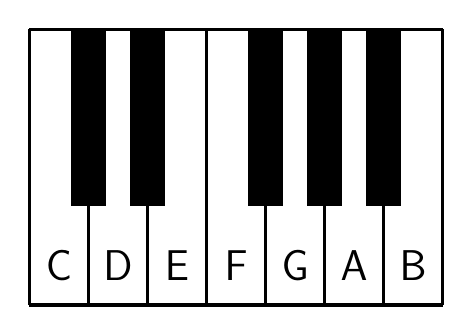
\begin{tikzpicture}[y=1cm/1.5,scale=0.75,transform shape]
    \draw[very thick,fill=white] (0,0) grid[xstep=1,ystep=7] (7,7);
    \foreach \i in {1,2,4,5,6}
      \fill (\i-.3,2.5) rectangle (\i+.3,7);
    \foreach \i [count=\j] in {C,D,E,F,G,A,B}
      \path (\j-.5,1) node[font=\huge\sffamily] {\i};
  \end{tikzpicture}
  \label{fig:music-notes:commands:note-values:letter}
\end{figure}
\begin{figure}[t]
  \centering
  \caption{Note name -- the number part}
  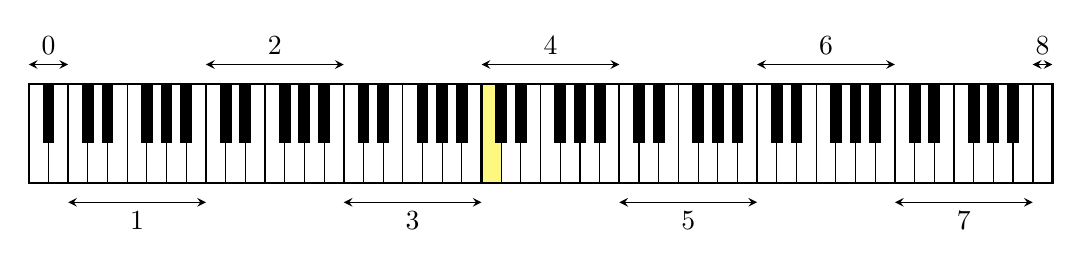
\begin{tikzpicture}[x=0.25cm,y=0.25cm,>=stealth]
    \fill[yellow!50] (23,0) rectangle (24,5);
    \draw (0,0) grid[xstep=1,ystep=5] (52,5);
    \draw[thick,shift={(2,0)}] (0,0) grid[xstep=7,ystep=5] (49,5);
    \draw[thick] (0,0) rectangle (2,5) (51,5) rectangle (52,0);
    \foreach \i in {1,...,7} {
      \foreach \j in {1,2,4,5,6} {
        \fill[shift={({2+(\i-1)*7},0)}] (\j-.3,2) rectangle (\j+.3,5);
      }
    }
    \fill (.7,2) rectangle (1.3,5);
    \foreach \i in {1,...,7} {
      \ifodd\i
        \draw[<->] ({(\i-1)*7+2},-1) -- ++ (7,0) node[midway,below] {\i};
      \else
        \draw[<->] ({(\i-1)*7+2},6) -- ++ (7,0) node[midway,above] {\i};
      \fi
    }
    \draw[<->] (0,6) -- (2,6) node[midway,above] {0};
    \draw[<->] (51,6) -- (52,6) node[midway,above] {8};
  \end{tikzpicture}
  \label{fig:music-notes:commands:note-values:number}
\end{figure}
Every white note is assigned to a `value', which is the \emph{scientific pitch 
notation} of that note. These values have two parts: the letter part and the 
number part:
\begin{itemize}
  \item The letter part can have seven values: |A|, |B|, |C|, \dots, |G|, 
  indicating the name of the note (\emph{do}, \emph{re}, \emph{mi}, \dots). (See 
  figure \ref{fig:music-notes:commands:note-values:letter}).
  \item The number part is a whole number between $0$ to $8$, indicating which 
  octave the note is in. (See figure \ref{fig:music-notes:commands:note-values:number}).
\end{itemize}
For example, \emph{F\"ur Elise} by Beethoven starts with an |E5| (a \emph{mi} at the 
5th octave).

We will only work with these values. To have black notes in your score, you can 
use \refCom*{tmappendaccidental} to add the accidentals.

The package will automatically detect which staff you are using, when you use 
these values.

\subsubsection{Whole notes}\label{sec:music-notes:commands:whole}
\begin{docCommand}{tmwhole}{\oarg{relative position}\marg{x-pos}\marg{note value list}\marg{name}}
  Add a set of whole notes at $x$-position \meta{x-pos}. Each value in the 
  comma-separated list \meta{note value list} corresponds to a note.

  \meta{name} can be left empty, but as in the staff naming, I strongly advise 
  you to find some name for each note set.

  The center of note with note value $x$ will be marked as coordinate 
  |(|\meta{name}|-|$x$|)|. For example, note |F5| will be marked as 
  |(|\meta{name}|-F5)|. Also, the point on the middle line of the staff which is 
  at \meta{x-pos} will be marked as |(|\meta{name}|-center)|.
\end{docCommand}
\begin{dispExample}
\begin{tmsinglestaff}
  \begin{tmstaff}{g}[]
    \tmwhole{3}{C4,E4,G4}{c-major}
    \tmwhole{5}{A4,C5,E5}{a-minor}
    \tmbarlineinline{4}
    \tmwhole{10}{G4,A4}{}
  \end{tmstaff}
\end{tmsinglestaff}
\end{dispExample}

This might not look good if two adjacent white notes are drawn (see the third 
note in the above example). One of the notes should be shifted to the right or 
to the left. In that case, you need to use two different \refCom*{tmwhole} 
commands for each of the `right' or `left' side and the center side. To specify 
on which side you are drawing, use either |left|, |center| or |right| for 
\meta{relative position}.

\begin{dispExample}
\begin{tmsinglestaff}
  \begin{tmstaff}{g}[]
    \tmwhole{3}{C4,E4,G4}{c-major}
    \tmwhole{5}{A4,C5,E5}{a-minor}
    \tmbarlineinline{4}
    \tmwhole{10}{G4}{}
    \tmwhole[right]{10}{A4}{}
    \tmwhole[left]{10}{F4}{}
  \end{tmstaff}
\end{tmsinglestaff}
\end{dispExample}
\subsubsection{Half notes}\label{sec:music-notes:commands:half}
\begin{docCommand}{tmhalf}{\oarg{relative position}\marg{x-pos}\marg{note value list}\marg{name}}
  Similar to \refCom*{tmwhole}. The stem points upwards if the `average' note 
  in the list is below the middle line, and downwards otherwise.
\end{docCommand}
\begin{docCommand}{tmhalf*}{\oarg{relative position}\marg{x-pos}\marg{note value list}\marg{name}}
  Identical to \refCom*{tmhalf}, only the stem direction is reversed. 
  \meta{relative position} works the same way as in \refCom*{tmwhole}.
\end{docCommand}
The end of the stem is marked as coordinate |(|\meta{name}|-tail)|. (This also 
applies to \refCom*{tmquarter}, \refCom*{tmeighth} and \refCom*{tmmorethaneighth}.)
\begin{dispExample}
\begin{tmsinglestaff}%
  \begin{tmstaff}{g}[]
    \tmhalf {2}{E4}{}\tmhalf {3}{F5}{}\tmhalf {4}{E4,F5}{}\tmhalf {5}{B4}{}
    \tmhalf*{6}{E4}{}\tmhalf*{7}{F5}{}\tmhalf*{8}{E4,F5}{}\tmhalf*{9}{B4}{}
    \tmhalf {11}{B4,G4}{}\tmhalf[right]{11}{C5}{}
    \tmhalf*{11}{G4}{}   \tmhalf*[left]{11}{F4}{}
  \end{tmstaff}%
\end{tmsinglestaff}
\end{dispExample}
\subsubsection{Quarter notes}\label{sec:music-notes:commands:quarter}
\begin{docCommand}{tmquarter}{\oarg{relative position}\marg{x-pos}\marg{note value list}\marg{name}}
  Similar to \refCom*{tmwhole}. The stem points upwards if the `average' note 
  in the list is below the middle line, and downwards otherwise.
\end{docCommand}
\begin{docCommand}{tmquarter*}{\oarg{relative position}\marg{x-pos}\marg{note value list}\marg{name}}
  Identical to \refCom*{tmquarter}, only the stem direction is reversed. 
  \meta{relative position} works the same way as in \refCom*{tmwhole}.
\end{docCommand}
\begin{dispExample}
\begin{tmsinglestaff}%
  \begin{tmstaff}{g}[]
    \tmquarter {2}{E4}{}\tmquarter {3}{F5}{}\tmquarter {4}{E4,F5}{}\tmquarter {5}{B4}{}
    \tmquarter*{6}{E4}{}\tmquarter*{7}{F5}{}\tmquarter*{8}{E4,F5}{}\tmquarter*{9}{B4}{}
    \tmquarter {11}{B4,G4}{}\tmquarter[right]{11}{C5}{}
    \tmquarter*{11}{G4}{}   \tmquarter*[left]{11}{F4}{}
  \end{tmstaff}%
\end{tmsinglestaff}
\end{dispExample}
\subsubsection{Eighth notes}\label{sec:music-notes:commands:eighth}
\begin{docCommand}{tmeighth}{\oarg{relative position}\marg{x-pos}\marg{note value list}\marg{name}}
  Similar to \refCom*{tmwhole}. The stem points upwards if the `average' note 
  in the list is below the middle line, and downwards otherwise.
\end{docCommand}
\begin{docCommand}{tmeighth*}{\oarg{relative position}\marg{x-pos}\marg{note value list}\marg{name}}
  Identical to \refCom*{tmeighth}, only the stem direction is reversed. 
  \meta{relative position} works the same way as in \refCom*{tmwhole}.
\end{docCommand}
\begin{dispExample}
\begin{tmsinglestaff}%
  \begin{tmstaff}{g}[]
    \tmeighth {2}{E4}{}\tmeighth {3}{F5}{}\tmeighth {4}{E4,F5}{}\tmeighth {5}{B4}{}
    \tmeighth*{6}{E4}{}\tmeighth*{7}{F5}{}\tmeighth*{8}{E4,F5}{}\tmeighth*{9}{B4}{}
    \tmeighth {11}{B4,G4}{}\tmeighth[right]{11}{C5}{}
    \tmeighth*{11}{G4}{}   \tmeighth*[left]{11}{F4}{}
  \end{tmstaff}%
\end{tmsinglestaff}
\end{dispExample}
\subsubsection{More than eighth notes}\label{sec:music-notes:commands:more-than-eighth}
The commands described in this section applies to every notes below the eighth 
notes, including the sixteenth note (semiquaver), the thirty-second note 
(demisemiquaver), etc.
\begin{docCommand}{tmmorethaneighth}{\oarg{relative position}\marg{x-pos}\marg{note value list}\marg{number of flags}\marg{name}}
  Similar to \refCom*{tmwhole}. The stem points upwards if the `average' note 
  in the list is below the middle line, and downwards otherwise.
\end{docCommand}
\begin{docCommand}{tmmorethaneighth*}{\oarg{relative position}\marg{x-pos}\marg{note value list}\marg{number of flags}\marg{name}}
  Identical to \refCom*{tmmorethaneighth}, only the stem direction is reversed. 
  \meta{relative position} works the same way as in \refCom*{tmwhole}.
\end{docCommand}
\begin{dispExample}
\begin{tmsinglestaff}%
  \begin{tmstaff}{g}[]
    \tmmorethaneighth{2}{F4}{2}{note-2}
    \tmmorethaneighth{3}{F4}{3}{note-3}
    \tmmorethaneighth{4}{F4}{4}{note-4}
    \tmmorethaneighth{5}{F4}{5}{note-5}
    \tmmorethaneighth{6}{F4}{6}{note-6}
  \end{tmstaff}%
\end{tmsinglestaff}
\end{dispExample}
\subsection{Beaming}\label{sec:music-notes:beam}
\begin{docEnvironment}[doclang/environment content=beaming note commands]{tmbeam}{}
  Add a beaming note series. All notes inside this environment are `beamed' 
  together, and all stems point {\bfseries upwards}.
\end{docEnvironment}
\begin{docEnvironment}[doclang/environment content=beaming note commands]{tmbeam*}{}
  Identical to \refEnv*{tmbeam}, only all stems point {\bfseries downwards}.
\end{docEnvironment}
\emph{All} notes to be beamed inside these environments need to be added using 
the following command (\refCom*{tmeighth}, \dots\ will simply not work):
\begin{docCommand}{tmbeamnote}{\oarg{relative position}\marg{x-pos}\marg{note value}\marg{number of flags}\marg{name}}
  Add a note to the beaming series. If \meta{number of flags} is $1$, it is an 
  eighth note, if \meta{number of flags} is $2$, it is a sixteenth note, and so 
  on.
\end{docCommand}
\begin{caution}
  {\bfseries\sffamily Important note:} Because of the algorithm working 
  behind the scene, you \emph{must} give a separate name to each \refCom*{tmbeamnote} 
  inside \refEnv*{tmbeam} or \refEnv*{tmbeam*}. Doing otherwise will result in 
  weird output.
\end{caution}
\begin{dispExample}
This is the incipit of a very famous piano piece. Can you name it?

\begin{tmsinglestaff}%
  \begin{tmstaff}{g}[p1]
    \tmtimesignature{1}{3}{8}
    \begin{tmbeam*}
      \tmbeamnote{1.75}{E5}{2}{}\tmbeamnote{2.5}{D5}{2}{a}
      \tmappendaccidental{a}{D5}{sharp}
    \end{tmbeam*}
    \tmbarlineinline{2.8}
    \begin{tmbeam*}
      \tmbeamnote{3.25}{E5}{2}{a}\tmbeamnote{4}{D5}{2}{b}\tmbeamnote{4.5}{E5}{2}{c}
      \tmbeamnote{5}{B4}{2}{d}\tmbeamnote{5.5}{D5}{2}{e}\tmbeamnote{6}{C5}{2}{f}
      \tmappendaccidental{b}{D5}{sharp}\tmappendaccidental{e}{D5}{natural}
    \end{tmbeam*}
    \tmbarlineinline{6.3}\tmeighth{6.75}{A4}{a}\tmadddot{a}{A4}
    \begin{tmbeam}
      \tmbeamnote{8}{C4}{2}{a}\tmbeamnote{8.5}{E4}{2}{b}\tmbeamnote{9}{A4}{2}{c}
    \end{tmbeam}
    \tmbarlineinline{9.3}\tmeighth{9.75}{B4}{a}\tmadddot{a}{B4}
    \begin{tmbeam}
      \tmbeamnote{10.75}{E4}{2}{a}\tmbeamnote{11.5}{G4}{2}{b}\tmbeamnote{12}{B4}{2}{c}
      \tmappendaccidental{b}{G4}{sharp}
    \end{tmbeam}
    \tmbarlineinline{12.3}\tmquarter{12.75}{C5}{a}\tmadddot{a}{C5}
  \end{tmstaff}%
  \tmbarlineendline{p1}{p1}%
\end{tmsinglestaff}
\end{dispExample}
\subsection{Commands for adding rests}\label{sec:music-notes:rests}
This package currently provides support for the following rests:
\begin{docCommand}{tmwholerest}{\oarg{shift}\marg{x-pos}}
  Add a whole rest at $x$-position \meta{x-pos}. \meta{shift} works just like in 
  \refCom*{tmkeysignature}.
\end{docCommand}
\begin{docCommand}{tmhalfrest}{\oarg{shift}\marg{x-pos}}
  Add a half rest at $x$-position \meta{x-pos}.
\end{docCommand}
\begin{docCommand}{tmquarterrest}{\oarg{shift}\marg{x-pos}}
  Add a quarter rest at $x$-position \meta{x-pos}.
\end{docCommand}
\begin{docCommand}{tmbelowquarterrest}{\oarg{shift}\marg{x-pos}\marg{number}}
  Add a rest at $x$-position \meta{x-pos}, whose value is below a quarter rest. 
  The rest has \meta{number} `flags': if \meta{number} is $1$, it is an eighth 
  rest, if \meta{number} is $2$, it is a sixteenth rest, and so on... Currently 
  \meta{number} must be an integer between |1| and |4|.
\end{docCommand}
\begin{docCommand}{tmeighthrest}{\oarg{shift}\marg{x-pos}}
  Identical to \refCom*{tmbelowquarterrest} where \meta{number} is $1$.
\end{docCommand}
\begin{docCommand}{tmsixteenthrest}{\oarg{shift}\marg{x-pos}}
  Identical to \refCom*{tmbelowquarterrest} where \meta{number} is $2$.
\end{docCommand}
\begin{docCommand}{tmthirtysecondrest}{\oarg{shift}\marg{x-pos}}
  Identical to \refCom*{tmbelowquarterrest} where \meta{number} is $3$.
\end{docCommand}
\begin{docCommand}{tmsixtyfourthrest}{\oarg{shift}\marg{x-pos}}
  Identical to \refCom*{tmbelowquarterrest} where \meta{number} is $4$.
\end{docCommand}
\begin{dispExample}
\begin{tmmultiplestaves}[0pt]%
  \begin{tmstaff}{g}
    \tmwholerest{2}\tmhalfrest{4}\tmquarterrest{6}
  \end{tmstaff}%
  \begin{tmstaff}{g}
    \tmbelowquarterrest{2}{1}\tmeighthrest{3}
    \tmbelowquarterrest{4}{2}\tmsixteenthrest{5}
    \tmbelowquarterrest{6}{3}\tmthirtysecondrest{7}
    \tmbelowquarterrest{8}{4}\tmsixtyfourthrest{9}
  \end{tmstaff}%
\end{tmmultiplestaves}
\end{dispExample}
\begin{dispExample}
\begin{tmsinglestaff}
  \begin{tmstaff*}
    \tmeighthrest[4]{3}\tmeighthrest[-4]{3}
    \tmwholerest[4]{6}\tmwholerest[-4]{6}
  \end{tmstaff*}
\end{tmsinglestaff}
\end{dispExample}
\subsection{Miscellaneous}\label{sec:music-notes:misc}
\subsubsection{Accidentals}\label{sec:music-notes:misc:accidentals}
\begin{docCommand}{tmappendaccidental}{\oarg{x-shift}\marg{note name}\marg{note value}\marg{type}}
  Add accidental \meta{type} to note of value \meta{note value} in 
  \meta{note name}. The accidental can be shifted in relative to it default 
  position using \meta{x-shift}.

  \meta{type} can have five values: |sharp|, |flat|, |double-sharp|, 
  |double-flat| and |natural|.
\end{docCommand}
\begin{dispExample}
\begin{tmsinglestaff}%
  \begin{tmstaff}{g}[]
    \tmquarter{2}{B4}{a}\tmquarter{3}{B4}{b}\tmquarter{4}{B4}{c}
    \tmquarter{5}{B4}{d}\tmquarter{6}{B4}{e}\tmquarter{9}{E4,G4,B4}{f}
    \tmappendaccidental{a}{B4}{sharp}
    \tmappendaccidental{b}{B4}{double-sharp}
    \tmappendaccidental{c}{B4}{flat}
    \tmappendaccidental{d}{B4}{double-flat}
    \tmappendaccidental{e}{B4}{natural}
    \tmappendaccidental{f}{E4}{sharp}
    \tmappendaccidental[-2mm]{f}{G4}{sharp}
    \tmappendaccidental[-4mm]{f}{B4}{sharp}
  \end{tmstaff}%
\end{tmsinglestaff}
\end{dispExample}
\subsubsection{Dots}\label{sec:music-notes:misc:dots}
\begin{docCommand}{tmadddot}{\oarg{x-shift}\marg{note name}\marg{note value}}
  Add a dot to note in \meta{note name} having \meta{note value}. You can use 
  \meta{x-shift} to shift it from the default position if necessary.
\end{docCommand}
\begin{docCommand}{tmadddot*}{\oarg{x-shift}\marg{note name}\marg{note value}\marg{number of dots}}
  Add \meta{number of dots} dot to note in \meta{note name} having 
  \meta{note value}. You can use \meta{x-shift} to shift it from the default 
  position if necessary.

  Basically \refCom*{tmadddot} is identical to \refCom*{tmadddot*} when 
  \meta{number of dots} is $1$.
\end{docCommand}
\begin{dispExample}
\begin{tmsinglestaff}%
  \begin{tmstaff}{g}[]
    \tmquarter{4}{A4}{a}\tmquarter{6}{B4}{b}\tmquarter{8}{C5}{c}
    \tmadddot{a}{A4}\tmadddot{b}{B4}\tmadddot*{c}{C5}{10}
  \end{tmstaff}%
\end{tmsinglestaff}
\end{dispExample}
\subsubsection{Articulations}\label{sec:music-notes:misc:articulations}
\begin{docCommand}{tmstaccato}{\oarg{shift}\marg{note name}}
  Add \emph{staccato} to note \meta{note name}.
\end{docCommand}
\begin{docCommand}{tmtenuto}{\oarg{shift}\marg{note name}}
  Add \emph{tenuto} to note \meta{note name}.
\end{docCommand}
\begin{docCommand}{tmaccentabove}{\oarg{shift}\marg{note name}}
  Add an accent to note \meta{note name} (one form of \emph{marcato}).
\end{docCommand}
\begin{docCommand}{tmstaccatissimo}{\oarg{shift}\marg{note name}}
  Add \emph{staccatissimo} to note \meta{note name}.
\end{docCommand}
\begin{docCommand}{tmmarcato}{\oarg{shift}\marg{note name}}
  Add \emph{marcato} to note \meta{note name}.
\end{docCommand}
\meta{shift} works just like in \refCom*{tmkeysignature}.
\begin{dispExample}
\begin{tmsinglestaff}
  \begin{tmstaff}{g}[]
    \tmquarter{2}{B4}{x}\tmstaccato{x}
    \tmquarter{3}{B4}{x}\tmstaccato[2]{x}
    \tmquarter{4}{B4}{x}\tmtenuto{x}
    \tmquarter{5}{B4}{x}\tmtenuto[2]{x}
    \tmquarter{6}{B4}{x}\tmaccentabove{x}
    \tmquarter{7}{B4}{x}\tmaccentabove[1]{x}
    \tmquarter{8}{B4}{x}\tmstaccatissimo{x}
    \tmquarter{9}{B4}{x}\tmstaccatissimo[1]{x}
    \tmquarter{10}{B4}{x}\tmmarcato{x}
    \tmquarter{11}{B4}{x}\tmmarcato[1]{x}
  \end{tmstaff}
\end{tmsinglestaff}
\end{dispExample}
You can also draw fermata:
\begin{docCommand}{tmfermata}{\oarg{shift}\marg{note name}}
  Add an `above-fermata' to \meta{note name}.
\end{docCommand}
\begin{docCommand}{tmfermata*}{\oarg{shift}\marg{note name}}
  Add a `below-fermata' to \meta{note name}.
\end{docCommand}
\begin{dispExample}
\begin{tmsinglestaff}
  \begin{tmstaff}{g}[]
    \tmquarter{5}{C4}{x}\tmfermata{x}
    \tmquarter{8}{C4}{x}\tmfermata*{x}
  \end{tmstaff}
\end{tmsinglestaff}
\end{dispExample}
\subsubsection{Ornaments}\label{sec:music-notes:misc:ornaments}
\begin{docCommand}{tmtrill}{\oarg{shift}\marg{note name}}
  Add a trill to note \meta{note name}.
\end{docCommand}
\begin{docCommand}{tmturn}{\oarg{shift}\marg{note name}}
  Add a turn to note \meta{note name}.
\end{docCommand}
\begin{docCommand}{tmmordent}{\oarg{shift}\marg{note name}}
  Add a `upper' mordent to note \meta{note name}.
\end{docCommand}
\begin{docCommand}{tmmordent*}{\oarg{shift}\marg{note name}}
  Add an `lower' mordent to note \meta{note name}.
\end{docCommand}
\begin{docCommand}{tmuppermordent}{\oarg{shift}\marg{note name}}
  Alias of \refCom*{tmmordent}.
\end{docCommand}
\begin{docCommand}{tmlowermordent}{\oarg{shift}\marg{note name}}
  Alias of \refCom*{tmmordent*}.
\end{docCommand}
\begin{dispExample}
%\usepackage{pgfplots}
%\pgfplotsset{compat=1.16}
\begin{tmsinglestaff}
  \begin{tmstaff}{g}
    \pgfplotsforeachungrouped \i in {2,4,6,8,10,12} {\tmquarter{\i}{C5}{q-\i}}
    \tmtrill{q-2}\tmturn{q-4}
    \tmmordent{q-6}\tmuppermordent{q-8}
    \tmmordent*{q-10}\tmlowermordent{q-12}
  \end{tmstaff}
\end{tmsinglestaff}
\end{dispExample}
\section{Other in-line stuffs}\label{sec:inline}
\subsection{Clefs}
You can add a clef in-line using the following commands:
\begin{docCommand}{tmgclef}{\oarg{shift}\marg{x-pos}}
  Add a treble clef at position \meta{x-pos}. The clef will be scaled down a bit 
  as per standards. \meta{shift} works like in \refCom*{tmkeysignature}.
\end{docCommand}
\begin{docCommand}{tmcclef}{\oarg{shift}\marg{x-pos}}
  Work like \refCom*{tmgclef}, but the clef is the alto clef.
\end{docCommand}
\begin{docCommand}{tmfclef}{\oarg{shift}\marg{x-pos}}
  Work like \refCom*{tmgclef}, but the clef is the bass clef.
\end{docCommand}
\begin{dispExample}
\begin{tmsinglestaff}
  \begin{tmstaff}{g}[]
    \tmquarter{3}{C4}{}
    \tmfclef{4}\tmquarter{5}{C4}{}
    \tmcclef{6}\tmquarter{7}{C4}{}
    \tmgclef{8}\tmquarter{9}{C4}{}
    \tmcclef[2]{10}\tmquarter{11}{C4}{}
  \end{tmstaff}
\end{tmsinglestaff}
\end{dispExample}
However, sometimes you don't want these clefs to be scaled. You can use the 
starred version of the mentioned commands.
\begin{docCommand}{tmgclef*}{\oarg{shift}\marg{x-pos}}
  Work like \refCom*{tmgclef}, but the clef is not scaled.
\end{docCommand}
\begin{docCommand}{tmcclef*}{\oarg{shift}\marg{x-pos}}
  Work like \refCom*{tmcclef}, but the clef is not scaled.
\end{docCommand}
\begin{docCommand}{tmfclef*}{\oarg{shift}\marg{x-pos}}
  Work like \refCom*{tmfclef}, but the clef is not scaled.
\end{docCommand}
\begin{dispExample}
\begin{tmsinglestaff}
  \begin{tmstaff}{g}[]
    \tmfclef*{4}\tmcclef*{6}\tmgclef*{8}\tmcclef*[2]{10}
  \end{tmstaff}%
\end{tmsinglestaff}
\end{dispExample}
Using \meta{shift}, we can have different versions of the three clefs. For example, 
we can have a tenor clef like this (the default distance from the starting point 
of a staff to its main clef is $2$mm):
\begin{dispExample}
\begin{tmsinglestaff}
  \begin{tmstaff*}[]
    \tmcclef*[2]{.2}
  \end{tmstaff*}
\end{tmsinglestaff}
\end{dispExample}
\section{Customizations}\label{sec:custom}
\begin{docCommand}{tmcolor}{}
  Set the color of everything. This is a predefined command with an initial value 
  |black|. You can redefine this command anywhere in your document to change 
  color of everything after that place.
\end{docCommand}
\begin{dispExample}
\begin{tmmultiplestaves}[0pt]%
  \begin{tmstaff}{g}
    \tmquarterrest{4}
    \renewcommand\tmcolor{red}
    \tmquarterrest{6}
    \renewcommand\tmcolor{black}
    \tmquarterrest{8}
  \end{tmstaff}%
  \begin{tmstaff}{g}
    \tmquarterrest{4}
    \begingroup
      \renewcommand\tmcolor{red}
      \tmquarterrest{6}
    \endgroup
    \tmquarterrest{8}
  \end{tmstaff}%
\end{tmmultiplestaves}
\end{dispExample}
\begin{docCommand}{tmnotelength}{}
  Set the length of the note stem of everything. This is a predefined command 
  with an initial value |6mm|. You can redefine this command anywhere in your 
  document to change the setting.
\end{docCommand}
\begin{dispExample}
\begin{tmsinglestaff}%
  \begin{tmstaff}{g}
    \begin{tmbeam}
      \renewcommand\tmnotelength{1.8cm}
      \tmbeamnote{4}{C4}{10}{a}\tmbeamnote{5}{D4}{10}{b}\tmbeamnote{6}{E4}{10}{c}
      \tmbeamnote{7}{F4}{10}{d}\tmbeamnote{8}{G4}{10}{e}\tmbeamnote{9}{A4}{10}{f}
    \end{tmbeam}
    \tmquarter*{10}{B4}{}
  \end{tmstaff}%
\end{tmsinglestaff}
\end{dispExample}
\section{\tikzname\ section}\label{sec:tikz}
The above sections don't require any prior knowledge about \tikzname. However, 
this package is based on \tikzname, and this section is dedicated to explain the 
\tikzname\ things that this package defines, so that you can use them more than 
just inside \refEnv*{tmsinglestaff} or \refEnv*{tmmultiplestaves}.
\subsection{Defined coordinates}\label{sec:tikz:coordinates}
\subsubsection{Staves}\label{sec:tikz:coordinates:staves}
When a staff is created, the middle line is the $x$-axis of the staff (i.e. 
every point on the middle line has $y$-coordinate $0$). The $y$-axis of the 
staff is the leftmost barline.

If the staff is named \meta{name}, three coordinates will be marked:
\begin{itemize}
  \item Coordinate |(|\meta{name}|-start)|: the leftmost point of the middle 
  line. 
  \item Coordinate |(|\meta{name}|-nw)|: the leftmost point of the top line.
  \item Coordinate |(|\meta{name}|-sw)|: the leftmost point of the bottom line.
\end{itemize}
The staves are all |remember picture| \tikzname\ pictures, so you can use these 
coordinates later in the document.
\begin{dispExample}
\begin{tmsinglestaff}
  \begin{tmstaff}{g}[my-staff]
    \path (my-staff-nw) node[above] {1} ++ (.5,.5) node[right] {\bfseries Allegro};
  \end{tmstaff}%
\end{tmsinglestaff}
\end{dispExample}
\subsubsection{Notes}\label{sec:tikz:coordinates:notes}
When a note set is drawn with name \meta{name}, the following coordinates are 
marked:
\begin{itemize}
  \item Coordinate |(|\meta{name}|-center)|: The point at the same $x$-position 
  that lies on the middle line of the staff.
  \item For each note having value \meta{note value}, the middle point of the 
  note is marked as coordinate |(|\meta{name}|-|\meta{note value}|)|.
  \item If the note has a stem, the ending point of that stem is marked as 
  |(|\meta{name}|-tail)|.
  \item In a beam, the coordinate at which the note stem intersects the beam 
  line is marked as coordinate |(|\meta{name}|-beamintersection)|.
\end{itemize}
\begin{dispExample}
\begin{tmsinglestaff}
  \begin{tmstaff}{g}[]
    \tmquarter*{3}{E5}{a}
    \begin{tmbeam}
      \tmbeamnote{7}{E5}{1}{b}\tmbeamnote{8}{D5}{1}{c}
    \end{tmbeam}
  \end{tmstaff}%
  \begin{tikzpicture}[remember picture,overlay,font=\sffamily\scriptsize]
    \fill[red] (a-center) circle (1.5pt) node[right] {a-center};
    \fill[green!50!black] (a-E5) circle (1.5pt) node[right] {a-E5};
    \fill[blue] (a-tail) circle (1.5pt) node[right] {a-tail};
    \fill[purple] (b-beamintersection) circle (1.5pt) node[left] {b-beamintersection};
  \end{tikzpicture}%
\end{tmsinglestaff}
\end{dispExample}
\subsection{Defined pics}\label{sec:tikz:pic}
\subsubsection{Clefs}\label{sec:tikz:pic:clefs}
Three pics are defined: |tm-g-clef| for the treble clef, |tm-c-clef| for the alto clef 
and |tm-f-clef| for the bass clef. 

\begin{dispExample}
\begin{tikzpicture}[scale=2,transform shape]
  \begin{scope}
    \pic {tm-g-clef};
    \draw[red,ultra thin] (-.2,0) -- (.7,0) (0,1) -- (0,-1);
    \draw[blue,ultra thin] (-.2,-.4) -- (.7,-.4);
  \end{scope}
  \begin{scope}[xshift=1.5cm]
    \pic {tm-c-clef};
    \draw[red,ultra thin] (-.2,0) -- (.7,0) (0,1) -- (0,-1);
    \draw[blue,ultra thin] (-.2,-.4) -- (.7,-.4) (-.2,.4) -- (.7,.4);
  \end{scope}
  \begin{scope}[xshift=3cm]
    \pic {tm-f-clef};
    \draw[red,ultra thin] (-.2,0) -- (.7,0) (0,1) -- (0,-1);
    \draw[blue,ultra thin] (-.2,.2) -- (.7,.2) (-.2,.4) -- (.7,.4);
  \end{scope}
\end{tikzpicture}
\end{dispExample}

The bounding boxes of |tm-c-clef| and |tm-f-clef| is set to the same height of 
|tm-g-clef| so that the distances between staves of different clefs can be 
equally positioned.
\subsubsection{Note heads and flags}\label{sec:tikz:pic:noteheads}
There are three types of note heads:

\begin{itemize}
  \item Whole note heads: there are three pics differing each other by the 
  relative position to the origin: |tm-whole-note-center|, |tm-whole-note-left|, 
  |tm-whole-note-right|:
\begin{dispExample}
\begin{tikzpicture}[scale=4,transform shape]
  \path (0,0)   pic       {tm-whole-note-center} 
        (0,.1)  pic[red]  {tm-whole-note-right}
        (0,-.1) pic[blue] {tm-whole-note-left};
\end{tikzpicture}
\end{dispExample}
  \item Half note heads: we also have three pics for each relative position:
\begin{dispExample}
\begin{tikzpicture}[scale=4,transform shape]
  \path (0,0)   pic       {tm-half-note-head-center} 
        (0,.1)  pic[red]  {tm-half-note-head-right}
        (0,-.1) pic[blue] {tm-half-note-head-left};
\end{tikzpicture}
\end{dispExample}
  \item Quarter note heads:
\begin{dispExample}
\begin{tikzpicture}[scale=4,transform shape]
  \path (0,0)   pic       {tm-quarter-note-head-center} 
        (0,.1)  pic[red]  {tm-quarter-note-head-right}
        (0,-.1) pic[blue] {tm-quarter-note-head-left};
\end{tikzpicture}
\end{dispExample}
\end{itemize}

There are two pics about note flags: the one for notes with stem heading up 
(|tm-note-flag-up|) and the one for notes with stem heading down (|tm-note-flag-down|).

\begin{dispExample}
\begin{tikzpicture}[scale=4,transform shape]
  \draw[red] (0,-.5) -- (0,0);
  \pic at (0,0) {tm-note-flag-up};
  \draw[red] (1,0) -- (1,-.5);
  \pic at (1,-.5) {tm-note-flag-down};
\end{tikzpicture}
\end{dispExample}
\subsubsection{Rests}\label{sec:tikz:pic:rests}
Whole rest and half rest can be easily drawn with a simple rectangle, so there 
are no pics for them. Internally this is how they are drawn when 
\refCom*{tmwholerest} and \refCom*{tmhalfrest} are executed:

\begin{dispExample}
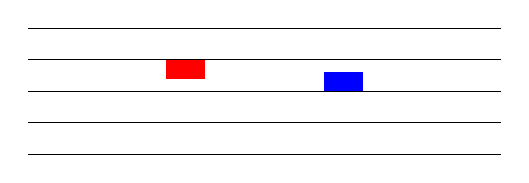
\begin{tikzpicture}[scale=2,transform shape]
  \foreach \i in {-.4,-.2,0,.2,.4} \draw (0,\i) -- (3,\i);
  \fill[red] (.875,.08) rectangle ++ (.25,.12);
  \fill[blue] (1.875,0) rectangle ++ (.25,.12);
\end{tikzpicture}
\end{dispExample}

Quarter rest is drawn using pic |tm-quarter-note-rest|:

\begin{dispExample}
\begin{tikzpicture}[scale=2,transform shape]
  \foreach \i in {-.4,-.2,0,.2,.4} \draw (0,\i) -- (2,\i);
  \pic[blue] at (1,0) {tm-quarter-note-rest};
\end{tikzpicture}
\end{dispExample}

For eighth rest and below, the pic name is |tm-|\meta{number}|-note-rest|, 
where \meta{number} is the number of `flags' in the rest notation. So 
|tm-1-note-rest| is the eighth rest, and so on. Currently \meta{number} must be 
either |1|, |2|, |3| or |4|.

\begin{dispExample}
\begin{tikzpicture}[scale=2,transform shape]
  \foreach \i in {-.4,-.2,0,.2,.4} \draw (0,\i) -- (5,\i);
  \foreach \i in {1,2,3,4} \pic[blue] at (\i,0) {tm-\i-note-rest};
\end{tikzpicture}
\end{dispExample}
\subsubsection{Numbers}\label{sec:tikz:pic:numbers}
The pics draw musical numbers, taken from the music font \emph{Maestro}. Digit 
\meta{x} has a pic named |tm-number-|\meta{x}. By default, these 
pics are $4$mm high.
\begin{dispExample}
\foreach \i in {0,...,9} {\tikz\pic {tm-number-\i};\quad}
\end{dispExample}
Position in relative to the origin:
\begin{dispExample}
\begin{tikzpicture}
  \pic[scale=4] at (0,0) {tm-number-6};
  \draw[ultra thin,red] (0,1) -- (0,-1) (-1,0) -- (1,0);
\end{tikzpicture}
\end{dispExample}
\subsubsection{Other time signature notations}\label{sec:tikz:pic:time-others}
You can also use pics |tm-common-time| and |tm-alla-breve-time|:
\begin{dispExample}
\begin{tikzpicture}[scale=2,transform shape]
  \path (0,0) pic {tm-common-time} (1,0) pic {tm-alla-breve-time};
  \draw[ultra thin,red] (-.5,0) -- (1.5,0);
  \foreach \i in {0,1} \draw[ultra thin,red] (\i,.5) -- (\i,-.5);
\end{tikzpicture}
\end{dispExample}
\subsubsection{Accidentals}\label{sec:tikz:pic:accidentals}
The pic name is the same with the name of the accidental: |tm-sharp|, |tm-flat|, 
|tm-natural|, |tm-double-sharp| and |tm-double-flat|.

\begin{dispExample}
\begin{tikzpicture}[scale=2,transform shape]
  \foreach \i in {0,1,2,3,4} \draw[ultra thin,red] (\i,-.5) -- (\i,.5);
  \draw[ultra thin,red] (-.5,0) -- (4.5,0);
  \path (0,0) pic {tm-sharp} (1,0) pic {tm-flat} (2,0) pic {tm-natural} 
        (3,0) pic {tm-double-sharp} (4,0) pic {tm-double-flat};
\end{tikzpicture}
\end{dispExample}

\printindex
\end{document}